\section{Arquitectura de la solució}
 
Aquesta secció descriu l'arquitectura tècnica del sistema de votació electrònica descentralitzat. L'objectiu és presentar una visió completa dels components del sistema, les seves responsabilitats, les relacions entre ells i les decisions de disseny que justifiquen cada elecció. L'arquitectura segueix el model C4 de Simon Brown, que permet representar el sistema a quatre nivells de detall creixent: context, contenidors, components i codi.
 
El principi fonamental que guia tot el disseny és l'eliminació del punt únic de fallada. Cap component individual del sistema ha de tenir la capacitat de modificar, censurar o invalidar un vot per si sol. Aquesta propietat es garanteix per construcció arquitectònica: la lògica electoral resideix íntegrament dins un contracte intel·ligent immutable desplegat a la xarxa Algorand, i cap servidor intermedi té accés a les claus privades dels votants ni al codi executable del contracte.
 
\subsection{Visió general del sistema (Nivell 1 — Context)}
 
El diagrama de context identifica els quatre actors externs que interactuen amb el sistema de votació descentralitzat:
 
\begin{enumerate}[label=\roman*.]
    \item \textbf{Votant}: persona física que emet el seu vot o proposa una elecció a través de la interfície web. Constitueix l'actor principal del sistema i l'únic que genera transaccions de votació.
    \item \textbf{Pera Wallet}: sistema de programari extern que gestiona les claus privades del votant. El sistema mai accedeix directament a aquestes claus; tota signatura criptogràfica es delega exclusivament a la cartera digital mitjançant el protocol WalletConnect.
    \item \textbf{Xarxa Algorand}: infraestructura blockchain on resideix el contracte intel·ligent de votació. En l'entorn de prototipat, es desplega sobre una xarxa local simulada amb AlgorKit; en un escenari de producció, es desplegaria a la Testnet o Mainnet d'Algorand.
    \item \textbf{Xarxa Ethereum}: emprada exclusivament com a notari públic. Un cop tancada l'elecció, un servei automàtic calcula el hash SHA-256 de l'estat final de l'escrutini i l'escriu a Ethereum (Sepolia Testnet) per garantir un ancoratge immutable i auditable de manera independent.
\end{enumerate}
 
Les comunicacions entre actors segueixen protocols estàndard: la interfície web es connecta al node Algorand via HTTPS/REST, la signatura dels vots es gestiona mitjançant WalletConnect, i l'ancoratge a Ethereum s'executa via JSON-RPC (Web3).

\begin{figure}[H]
    \centering
    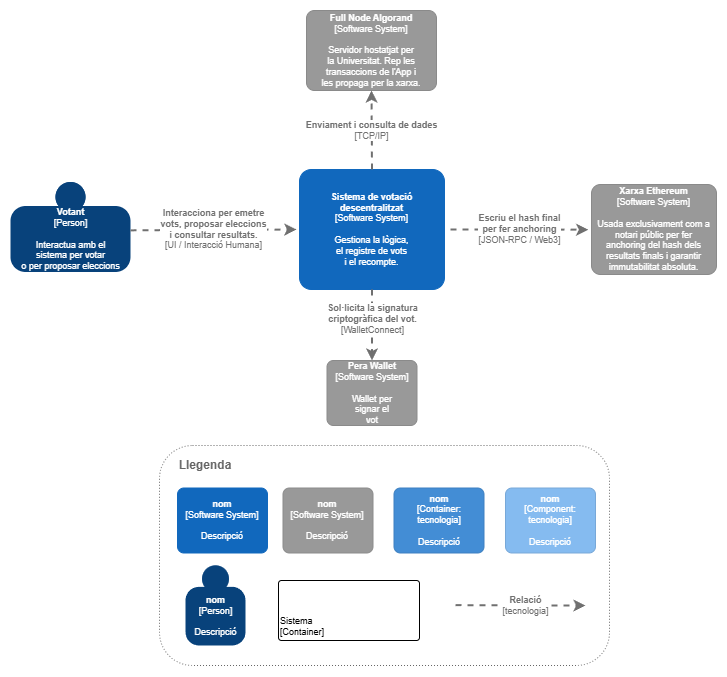
\includegraphics[width=0.85\textwidth]{images/c4-n1.png} 
    \caption{Primer nivell del model C4.}
    \label{fig:c4-nivell-1}
\end{figure}
 
\subsection{Contenidors del sistema (Nivell 2)}
 
El sistema es descompon en cinc contenidors principals, cadascun amb una responsabilitat ben delimitada i un acoblament mínim amb la resta:
 
\subsubsection{Aplicació d'escriptori (Front-end)}
 
Aplicació web que el votant descarrega i executa localment. Desenvolupada amb React, és responsable de renderitzar la interfície d'usuari, mostrar les eleccions actives, empaquetar el vot en format de transacció Algorand (ApplicationCall) i enviar-lo al node. L'aplicació no emmagatzema cap dada sensible i opera com un client lleuger (\textit{thin client}) que delega tota la lògica de negoci al contracte intel·ligent.
 
El flux d'interacció de l'usuari segueix una seqüència de quatre passos: (1) l'usuari tria l'opció de vot, (2) l'aplicació empaqueta el vot en format JSON, (3) sol·licita la signatura criptogràfica a la cartera digital i (4) envia la transacció signada al node complet d'Algorand perquè la propagui a la xarxa.
 
\subsubsection{Node Complet d'Algorand}
 
Servidor hostatjat per la universitat (o, en un escenari productiu, per les entitats participants) que rep les transaccions de l'aplicació web i les propaga per la xarxa blockchain. Implementat en Go, exposa una API REST estàndard compatible amb l'Algorand SDK. La seva funció és exclusivament la de punt d'entrada a la xarxa: no conté lògica de negoci pròpia ni té accés a les claus dels votants.
 
En el context del prototip acadèmic, es desplega un únic node local mitjançant AlgorKit dins un contenidor Docker. En una arquitectura de producció, múltiples entitats (universitats, partits, observadors) mantindrien cadascuna un node complet per garantir la redundància i la descentralització real de la infraestructura.
 
\subsubsection{Smart Contract de Votació}
 
Lògica immutable desplegada a la xarxa Algorand, escrita en PyTeal i compilada a TEAL (Transaction Execution Approval Language). Constitueix el nucli del sistema i la peça que elimina la necessitat de confiança en cap autoritat central. Les seves responsabilitats són:
 
\begin{enumerate}[label=\roman*.]
    \item Generació i emmagatzematge de propostes de votació.
    \item Validació del cens electoral (verificació que l'adreça del votant pertany a la llista blanca).
    \item Prevenció del doble vot mitjançant Local State.
    \item Gestió del cicle de vida de l'elecció (dates d'inici i finalització).
    \item Recompte automàtic i transparent dels vots.
\end{enumerate}
 
L'estat del contracte s'emmagatzema emprant dos mecanismes natius d'Algorand: \textbf{Box Storage} per guardar les propostes i el recompte global de vots, i \textbf{Local State} per registrar si un votant concret ja ha exercit el seu dret, evitant així el doble vot sense revelar l'opció seleccionada.
 
\subsubsection{Servei d'Anchoring}
 
Script automatitzat escrit en Python que, un cop el contracte intel·ligent marca una elecció com a ``Tancada'', llegeix l'estat final del recompte des del node d'Algorand, calcula el hash SHA-256 del resultat complet i l'escriu a la xarxa pública d'Ethereum (Sepolia Testnet) mitjançant una transacció. Aquesta operació crea un segell de temps criptogràfic incorruptible que qualsevol auditor pot verificar de manera independent sense necessitat d'accedir a la xarxa d'Algorand.
 
El servei s'executa de forma desatesa i no requereix intervenció humana. L'única clau privada que gestiona és la del compte d'Ethereum destinat exclusivament a l'ancoratge, finançat amb criptomoneda de prova obtinguda de faucets públiques.
 
\subsubsection{Pera Wallet (sistema extern)}
 
Cartera digital mòbil de l'ecosistema Algorand que actua com a custòdia exclusiva de les claus privades del votant. El sistema interactua amb Pera Wallet a través del protocol WalletConnect: l'aplicació web genera un codi QR, l'usuari l'escaneja, i la cartera retorna la transacció signada criptogràficament sense que la clau privada abandoni mai el dispositiu mòbil de l'elector.

\begin{figure}[H]
    \centering
    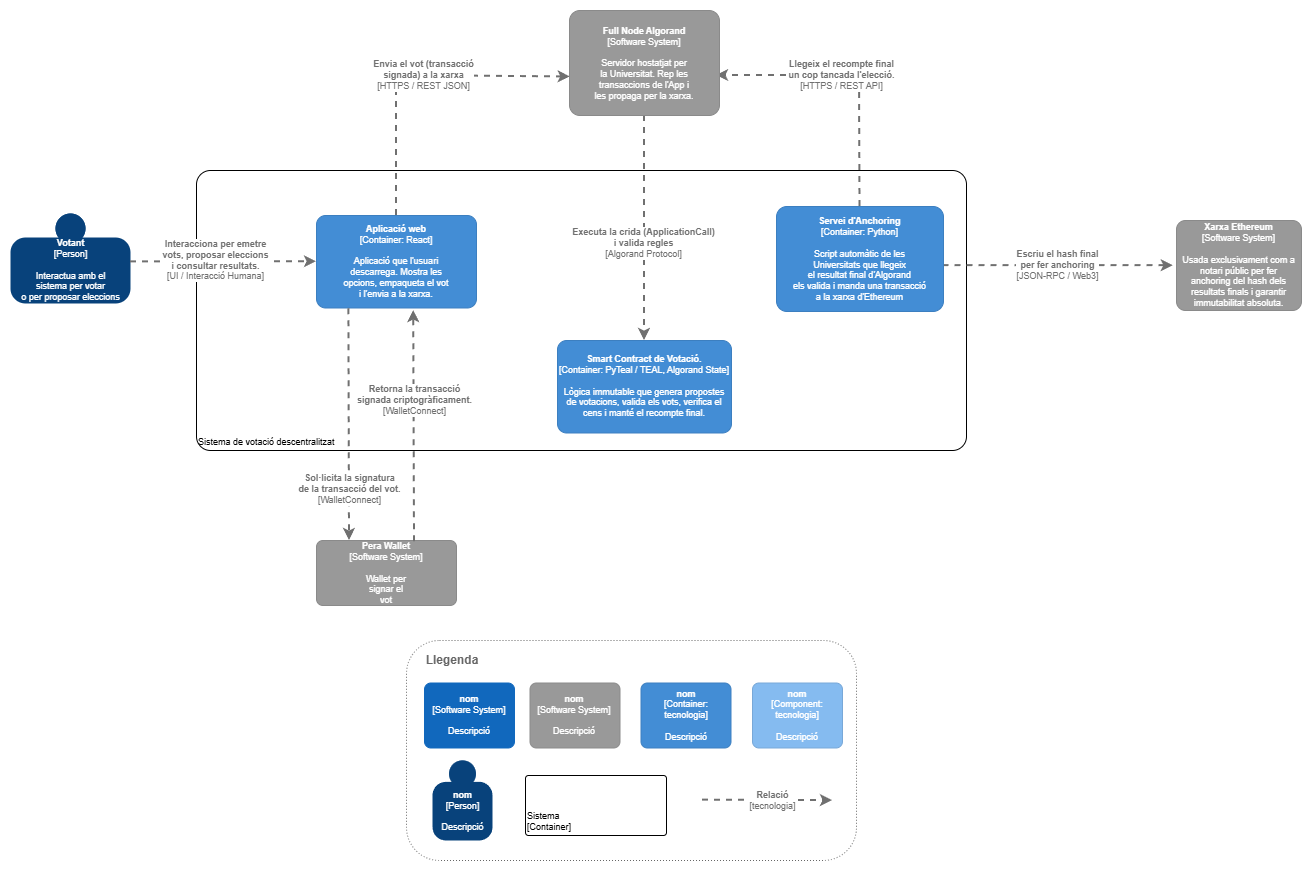
\includegraphics[width=0.85\textwidth]{images/c4-n2.png} 
    \caption{Segon nivell del model C4.}
    \label{fig:c4-nivell-1}
\end{figure}

\subsection{Components interns (Nivell 3)}
 
A continuació es detalla la descomposició interna dels dos contenidors més complexos del sistema: l'aplicació d'escriptori i el contracte intel·ligent.
 
\subsubsection{Components de l'aplicació d'escriptori}
 
L'aplicació React es descompon en quatre components principals amb responsabilitats clarament separades:
 
\begin{enumerate}[label=\roman*.]
    \item \textbf{Gestor d'interfície} (\textit{React Components}): renderitza les pantalles de l'aplicació, incloent-hi la llista d'eleccions actives, la papereta de vot i el formulari de creació de noves propostes d'eleccions.
 
    \item \textbf{Controlador d'estat} (\textit{Redux / React Context}): emmagatzema l'estat local de l'aplicació, com ara les dades de les eleccions descarregades des del node i l'estat de connexió de la cartera digital. Actua com a font única de veritat (\textit{single source of truth}) per a tota la interfície.
 
    \item \textbf{Mòdul WalletConnect} (\textit{WalletConnect SDK}): gestiona la sessió amb Pera Wallet, genera el codi QR per establir la connexió i envia les sol·licituds de signatura a l'usuari. Encapsula tota la complexitat del protocol de comunicació amb la cartera.
 
    \item \textbf{Generador de transaccions} (\textit{Algorand JS SDK — algosdk}): tradueix les accions de l'usuari (``Votar opció A'' o ``Proposar elecció X'') en transaccions \textit{byte-code} d'Algorand (ApplicationCall) a punt per ser signades. Aquesta capa d'abstracció garanteix que la resta de l'aplicació no necessita conèixer els detalls de baix nivell del protocol Algorand.
\end{enumerate}
 
\subsubsection{Components del Smart Contract}
 
El contracte intel·ligent es descompon internament en cinc mòduls lògics:
 
\begin{enumerate}[label=\roman*.]
    \item \textbf{Enrutador principal} (\textit{PyTeal Cond}): punt d'entrada del contracte. Rep cada transacció i, segons els arguments de l'ApplicationCall, la redirigeix al mòdul de votació, al de propostes o al generador d'eleccions. Implementa el patró \textit{Router} per centralitzar el control del flux d'execució.
 
    \item \textbf{Lògica de propostes} (\textit{PyTeal}): revisa que l'usuari pugui realitzar propostes, verifica que la proposta no existeixi prèviament (retornant error en cas contrari) i, si és nova, defineix les dates d'inici i finalització, el nom de la proposta, els participants i els elements a ser elegits.
 
    \item \textbf{Lògica de votació} (\textit{PyTeal}): comprova que l'elecció estigui activa (dins la finestra temporal), verifica que l'usuari no hagi votat ja consultant el Local State i, si totes les condicions es compleixen, incrementa el comptador de l'opció triada al Box Storage.
 
    \item \textbf{Generador d'eleccions} (\textit{PyTeal}): llegeix l'estat del contracte i, si una proposta ha assolit un llindar determinat de vots favorables, genera automàticament les eleccions corresponents. Implementa la lògica de transició entre la fase de proposta i la fase electoral.
 
    \item \textbf{Emmagatzematge d'estat} (\textit{Algorand Box Storage \& Local State}): base de dades del contracte. Guarda les propostes (Box Storage), el recompte de vots per elecció (Global/Box) i el registre individual de qui ha votat (Local State per evitar el doble vot).
\end{enumerate}
 
 
% ===========================================================================
%   SECCIÓ 9 — TECNOLOGIES I SOFTWARE DE TERCERS
% ===========================================================================
\section{Tecnologies i software de tercers}
 
El sistema s'ha construït emprant exclusivament eines de codi obert i plataformes gratuïtes, en coherència amb el requisit de projecte d'incórrer en zero despesa econòmica (secció 3.3.3 del document d'abast). Cada tecnologia s'ha seleccionat atenent a criteris de maduresa, documentació disponible, compatibilitat amb l'ecosistema Algorand i accessibilitat per a l'equip de desenvolupament. A continuació es descriuen les tecnologies emprades, agrupades per capa del sistema.
 
\subsection{Capa de blockchain i contractes intel·ligents}
 
\subsubsection{Algorand (protocol de consens)}
 
Algorand és la xarxa blockchain seleccionada com a infraestructura sobirana del sistema de votació. Utilitza un mecanisme de consens basat en Pure Proof of Stake (PPoS) combinat amb una Funció Aleatòria Verificable (VRF) que garanteix que la selecció de validadors és aleatòria, impredictible i verificable criptogràficament. Les seves propietats fonamentals per al projecte són: finalitat immediata de les transaccions (sense possibilitat de \textit{forks}), comissions de transacció negligibles (0,001 ALGO), i suport natiu per a contractes intel·ligents amb emmagatzematge d'estat (Global State, Local State i Box Storage).
 
La decisió d'emprar Algorand en lloc d'Ethereum per a la lògica de votació es justifica per tres raons: (1) la finalitat instantània elimina la incertesa sobre si un vot ha estat confirmat, (2) el cost per transacció és ordres de magnitud inferior al gas d'Ethereum, fent viable un sistema on cada vot és una transacció, i (3) el model d'emmagatzematge natiu (Box Storage) permet estructures de dades complexes directament al contracte sense necessitat de mapejar tot a \textit{storage slots} de 256 bits.
 
\subsubsection{PyTeal / TEAL}
 
PyTeal és una llibreria de Python que permet escriure contractes intel·ligents per a Algorand emprant sintaxi Python nativa, que posteriorment es compila a TEAL (\textit{Transaction Execution Approval Language}), el llenguatge d'assembler de la màquina virtual d'Algorand (AVM). L'elecció de PyTeal per sobre d'alternatives com Puya (Algorand Python) es basa en la major maduresa de la seva documentació i la disponibilitat d'exemples dins la comunitat, factors crítics donada la corba d'aprenentatge prevista a la gestió de riscos (secció 6.4).
 
Tot el codi dels contractes (lògica de propostes, votació, generació d'eleccions i enrutament) s'escriu en PyTeal i es compila a TEAL abans del desplegament. Aquesta separació entre el llenguatge de desenvolupament (Python) i el d'execució (TEAL) facilita les proves unitàries i la lectura del codi per part d'auditors.
 
\subsubsection{AlgorKit (AlgoKit)}
 
AlgorKit és l'eina oficial de la Fundació Algorand per a la gestió del cicle de vida complet dels projectes blockchain: creació de l'entorn local, desplegament de contractes, execució de proves i interacció amb la xarxa. En el context d'aquest projecte, s'empra per aixecar una xarxa Algorand local simulada dins un contenidor Docker amb una única comanda, permetent iterar ràpidament sobre el codi dels contractes sense incórrer en costos de xarxa.
 
AlgorKit proporciona comptes prefabricats amb saldos de prova, un indexer local per a consultes, i una CLI que automatitza les tasques repetitives de desplegament. Constitueix la peça clau per complir el requisit de reproducibilitat (secció 3.2.1): qualsevol membre de l'equip pot replicar l'entorn exacte clonant el repositori i executant \texttt{algokit localnet start}.
 
\subsection{Capa de front-end}
 
\subsubsection{React}
 
React és la llibreria de JavaScript seleccionada per al desenvolupament de la interfície d'usuari. La seva arquitectura basada en components reactius i el seu model de flux de dades unidireccional permeten mantenir una separació neta entre la presentació visual i la lògica d'estat de l'aplicació. L'equip compta amb experiència prèvia en React (secció 5.2), la qual cosa redueix la corba d'aprenentatge i permet concentrar l'esforç en la integració blockchain.
 

\subsubsection{Algorand JavaScript SDK (algosdk)}
 
La llibreria oficial \texttt{algosdk} permet a l'aplicació web construir, signar i enviar transaccions d'Algorand des del navegador. S'empra per traduir les accions de l'usuari en transaccions \textit{ApplicationCall} byte-code compatibles amb el contracte intel·ligent. La versió emprada suporta la construcció de transaccions atòmiques (grups de transaccions) i la interacció amb Box Storage.
 
\subsubsection{WalletConnect SDK}
 
WalletConnect és el protocol de comunicació estàndard entre aplicacions web (dApps) i carteres digitals mòbils. El SDK s'integra a l'aplicació React per generar codis QR de connexió, establir sessions xifrades amb Pera Wallet i enviar sol·licituds de signatura. Totes les comunicacions entre l'aplicació i la cartera es xifren mitjançant un pont (\textit{bridge}) independent, garantint que la clau privada del votant mai transita per la xarxa de l'aplicació.
 
\subsection{Capa d'anchoring i auditoria}
 
\subsubsection{Ethereum (Sepolia Testnet)}
 
La xarxa pública d'Ethereum s'empra exclusivament com a notari públic extern. El servei d'anchoring escriu el hash SHA-256 dels resultats finals a la Sepolia Testnet, creant un registre verificable de manera independent per qualsevol auditor amb accés a un explorador de blocs d'Ethereum. La selecció de Sepolia en lloc d'altres testnets (Goerli, ja obsoleta) segueix la recomanació oficial de la Fundació Ethereum per a aplicacions de prova.
 
\subsubsection{Web3.py}
 
Llibreria de Python que proporciona la interfície de comunicació amb la xarxa Ethereum mitjançant el protocol JSON-RPC. S'empra dins el servei d'anchoring per construir i enviar la transacció que conté el hash de l'escrutini. La seva compatibilitat nativa amb Sepolia i la seva àmplia documentació la fan la solució més directa per a l'escriptura de dades a Ethereum des d'un script Python.
 
\subsection{Capa d'infraestructura i desplegament}
 
\subsubsection{Docker}
 
Docker és l'eina central de contenidorització del projecte. Permet empaquetar tots els serveis del sistema (node Algorand, servidor front-end, servei d'anchoring) en contenidors independents i reproduïbles. Cada component es defineix en un \texttt{Dockerfile} propi i l'orquestració del conjunt es gestiona amb \texttt{docker-compose}, garantint que qualsevol desenvolupador o avaluador pugui desplegar el sistema complet amb una única comanda.
 
\subsubsection{Git i GitHub}
 
El sistema de control de versions es gestiona amb Git, i el repositori central s'allotja a GitHub. L'estratègia de branques segueix el model Trunk Based Development descrit a la secció 7.2 del document d'abast, amb branques de funcionalitat curtes que s'integren a \texttt{main} mitjançant Pull Requests revisades.
 
\subsection{Resum de tecnologies}
 
La taula~\ref{tab:tecnologies} resumeix totes les tecnologies emprades, la seva capa dins l'arquitectura i la seva funció específica.
 
\begin{table}[H]
\centering
\small
\begin{tabularx}{\textwidth}{l l X}
\toprule
\textbf{Tecnologia} & \textbf{Capa} & \textbf{Funció dins el sistema} \\
\midrule
Algorand (PPoS/VRF) & Blockchain & Xarxa sobirana on resideix el contracte de votació \\
PyTeal / TEAL & Blockchain & Escriptura i compilació dels contractes intel·ligents \\
AlgorKit & Blockchain & Entorn local simulat i CLI de desplegament \\
React & Front-end & Interfície d'usuari de l'aplicació de votació \\
Redux / Context & Front-end & Gestió centralitzada de l'estat de l'aplicació \\
algosdk (JS) & Front-end & Construcció de transaccions Algorand des del navegador \\
WalletConnect SDK & Front-end & Protocol de comunicació segura amb Pera Wallet \\
Pera Wallet & Externa & Custòdia de claus privades i signatura de transaccions \\
Ethereum (Sepolia) & Anchoring & Notari públic per a l'ancoratge del hash dels resultats \\
Web3.py & Anchoring & Interfície Python per a la interacció amb Ethereum \\
Docker & Infraestructura & Contenidorització i reproducibilitat de l'entorn \\
Git / GitHub & Infraestructura & Control de versions i col·laboració \\
\bottomrule
\end{tabularx}
\caption{Resum de tecnologies i software de tercers emprats al projecte}
\label{tab:tecnologies}
\end{table}
 
 
% ===========================================================================
%   SECCIÓ 10 — DECISIONS TÈCNIQUES (PATRONS DE DISSENY)
% ===========================================================================
\section{Decisions tècniques (patrons de disseny)}
 
Les decisions tècniques del projecte no responen a criteris arbitraris, sinó a la necessitat de resoldre problemes concrets derivats dels requisits funcionals i no funcionals establerts a la secció 3 del document d'abast. Cada decisió es presenta juntament amb el problema que resol, les alternatives considerades i la justificació de l'opció triada.
 
\subsection{Patró Router per al contracte intel·ligent}
 
\textbf{Problema}: un contracte intel·ligent d'Algorand rep totes les transaccions a través d'un únic punt d'entrada (l'Approval Program). Cal un mecanisme per distingir si una transacció és un vot, una proposta, una consulta de resultats o una sol·licitud de generació d'eleccions.
 
\textbf{Solució}: s'implementa un enrutador principal (patró \textit{Router}) al començament del codi PyTeal que inspeccionaria els arguments de l'ApplicationCall (\texttt{Txn.application\_args[0]}) i, mitjançant una estructura condicional (\texttt{Cond}), redirigeix l'execució al mòdul corresponent: lògica de votació, lògica de propostes o generador d'eleccions.
 
\textbf{Justificació}: aquest patró centralitza el control de flux, facilita l'extensibilitat del contracte (afegir noves funcionalitats sense modificar els mòduls existents) i millora la llegibilitat del codi, ja que cada mòdul gestiona una única responsabilitat. A més, segueix el principi de responsabilitat única (\textit{Single Responsibility Principle}) dins les restriccions de la AVM, que no permet herència ni modularització a nivell de fitxers.
 
\subsection{Separació d'estat: Box Storage vs. Local State}
 
\textbf{Problema}: el contracte necessita emmagatzemar dos tipus de dades amb requisits d'accés molt diferents: (1) informació global compartida (propostes d'elecció, recomptes de vots, dates) i (2) informació individual per votant (si ha votat o no en una elecció concreta).
 
\textbf{Solució}: les dades globals s'emmagatzemen en \textbf{Box Storage}, que ofereix espai d'emmagatzematge de mida variable associat al contracte, adequat per a estructures de dades complexes com llistes de propostes o mapeigs de recompte. Les dades individuals de cada votant es registren al \textbf{Local State}, que és un espai d'emmagatzematge lligat al compte de l'usuari que ha fet \textit{opt-in} al contracte, perfecte per registrar un \textit{flag} booleà de ``ha votat''.
 
\textbf{Justificació}: aquesta separació explota les propietats natives d'Algorand de manera òptima. El Local State permet verificar el doble vot amb una sola lectura (O(1)) sense necessitat d'iterar una llista de votants al Box Storage, cosa que seria inviable dins els límits d'opcode de la AVM. A més, el Local State és privat del compte de l'usuari, proporcionant una capa addicional de separació entre la identitat del votant i la seva acció.
 
\subsection{Thin Client: delegació completa de lògica al contracte}
 
\textbf{Problema}: si l'aplicació web conté lògica de validació duplicada (per exemple, comprovar el cens o verificar dates), existeix un risc de discrepància entre el comportament del front-end i el del contracte, a més de crear un vector d'atac si un usuari maliciós modifica el codi client.
 
\textbf{Solució}: l'aplicació d'escriptori opera com un \textit{Thin Client} que no implementa cap regla de negoci. Tota la validació (cens, doble vot, finestra temporal, increment de comptadors) resideix exclusivament al contracte intel·ligent. El front-end es limita a construir transaccions, sol·licitar signatures i mostrar resultats.
 
\textbf{Justificació}: en un sistema on la confiança es resol per disseny, el codi executable de referència ha de ser únic i residir a la blockchain. Si la validació del cens estigués al front-end, un atacant podria modificar el JavaScript i intentar emetre transaccions invàlides. Amb el model \textit{Thin Client}, qualsevol transacció que no compleixi les regles del contracte serà rebutjada per la xarxa independentment del que faci l'aplicació client.
 
\subsection{Patró Single Source of Truth per a l'estat del front-end}
 
\textbf{Problema}: múltiples components de React necessiten accedir a les mateixes dades (llista d'eleccions, estat de la connexió de la wallet, fase del procés de votació). Si cada component manté el seu propi estat, les inconsistències són inevitables.
 
\textbf{Solució}: tot l'estat de l'aplicació es centralitza en un únic \textit{store} gestionat per Redux (o alternativament React Context amb \texttt{useReducer}). Els components accedeixen a les dades via selectors i disparen accions per modificar-les, seguint un flux de dades unidireccional estricte.
 
\textbf{Justificació}: el patró \textit{Single Source of Truth} és especialment crític en aplicacions que interactuen amb blockchain, on l'estat pot canviar de manera asíncrona (per exemple, un vot que es confirma després d'uns segons). Un contenidor d'estat centralitzat permet gestionar correctament les transicions d'estat, mostrar indicadors de càrrega i garantir que la interfície reflecteix fidelment l'estat real de la xarxa.
 
\subsection{Signatura delegada i principi de mínim privilegi}
 
\textbf{Problema}: el sistema necessita que les transaccions estiguin signades criptogràficament amb la clau privada del votant, però cap component de la infraestructura pot tenir accés a aquesta clau.
 
\textbf{Solució}: s'aplica el principi de mínim privilegi delegant completament la signatura a Pera Wallet mitjançant WalletConnect. L'aplicació web construeix la transacció (no signada), l'envia a la cartera, i rep de tornada la transacció signada per propagar-la al node. En cap moment la clau privada abandona el dispositiu mòbil del votant.
 
\textbf{Justificació}: la gestió incorrecta de claus privades és el vector d'atac més comú en aplicacions descentralitzades. Delegar la signatura a una cartera especialitzada elimina de soca-rel la possibilitat que un servidor compromès o un error al front-end exposi les credencials del votant. A més, aquest model és transparent per a l'usuari: l'acció de signar un vot es percep com una confirmació al mòbil, similar a la validació biomètrica d'una aplicació bancària.
 
\subsection{Ancoratge extern (Cross-chain Anchoring)}
 
\textbf{Problema}: el contracte d'Algorand és immutable per disseny, però un atacant sofisticat podria argumentar que la xarxa local (o fins i tot una Testnet) no ofereix suficients garanties de permanència. Cal un mecanisme que proporcioni un segell de temps independent i verificable fora de l'ecosistema Algorand.
 
\textbf{Solució}: un cop tancada l'elecció, un servei automàtic calcula el hash SHA-256 de l'estat final (resultats complets de l'escrutini) i l'escriu com a dada (\textit{calldata}) a una transacció d'Ethereum a la Sepolia Testnet. Qualsevol auditor pot verificar posteriorment que el hash publicat a Ethereum coincideix amb el hash calculable a partir de l'estat d'Algorand.
 
\textbf{Justificació}: aquest patró, conegut com a \textit{cross-chain anchoring} o \textit{state anchoring}, proporciona una capa addicional de seguretat i auditabilitat. Ethereum, com a xarxa pública amb milers de nodes independents, actua com a notari públic extern. Si un atacant modifiqués l'estat d'Algorand (cosa ja criptogràficament inviable), el hash resultant no coincidiria amb el publicat a Ethereum, fent evident qualsevol manipulació.
 
\subsection{Resum de decisions tècniques}
 
La taula~\ref{tab:decisions} sintetitza les decisions de disseny principals i la seva traçabilitat amb els requisits del sistema.
 
\begin{table}[H]
\centering
\small
\begin{tabularx}{\textwidth}{l l X}
\toprule
\textbf{Decisió} & \textbf{Patró} & \textbf{Requisit que resol} \\
\midrule
Enrutador del contracte & Router & RF 3.1.2, 3.1.3, 3.1.6 \\
Separació Box/Local State & Strategy (Storage) & RF 3.1.2 (doble vot), 3.1.4 \\
Thin Client & Client-Server & RNF 3.2.5 (seguretat) \\
Store centralitzat & Single Source of Truth & RNF 3.2.4 (usabilitat) \\
Signatura delegada & Mínim privilegi & RNF 3.2.5 (credencials) \\
Ancoratge a Ethereum & Cross-chain Anchoring & RF 3.1.7 (immutabilitat) \\
\bottomrule
\end{tabularx}
\caption{Traçabilitat entre decisions tècniques i requisits del sistema}
\label{tab:decisions}
\end{table}
 
 
% ===========================================================================
%   SECCIÓ 11 — ESTRATÈGIA DE DESPLEGAMENT
% ===========================================================================
\section{Estratègia de desplegament}
 
L'estratègia de desplegament defineix com el sistema es construeix, es posa en marxa i es valida en cada una de les seves fases. Donada la naturalesa acadèmica del projecte i la restricció de zero cost econòmic, tot el desplegament es basa en entorns locals simulats i xarxes de prova públiques gratuïtes.
 
\subsection{Entorn de desplegament local}
 
L'entorn de desenvolupament i proves es basa en una xarxa Algorand local simulada, gestionada íntegrament per AlgorKit i orquestrada amb Docker. L'objectiu és que qualsevol desenvolupador o avaluador pugui reproduir el sistema complet amb un esforç mínim de configuració.
 
El procés de posada en marxa segueix una seqüència determinista:
 
\begin{enumerate}[label=\roman*.]
    \item \textbf{Inicialització de la xarxa}: s'executa \texttt{algokit localnet start}, que aixeca un node Algorand complet, un indexer i un KMD (\textit{Key Management Daemon}) dins contenidors Docker. Aquesta comanda crea automàticament comptes de prova amb saldos suficients per a les transaccions.
    \item \textbf{Desplegament del contracte}: es compila el codi PyTeal a TEAL i es desplega el contracte intel·ligent a la xarxa local mitjançant la CLI d'AlgorKit (\texttt{algokit deploy}). El procés retorna l'identificador (App ID) del contracte desplegat.
    \item \textbf{Configuració del cens}: un script de Python pobla el contracte amb una llista blanca d'adreces de prova que simulen el cens electoral autoritzat.
    \item \textbf{Arrancada del front-end}: l'aplicació React s'inicia amb \texttt{npm start} (o dins un contenidor Docker propi) i es configura perquè apunti al node local d'Algorand i a l'App ID del contracte desplegat.
    \item \textbf{Verificació integral}: l'equip de QA executa la bateria de proves automatitzades per confirmar que tot el flux (connexió de wallet, emissió de vot, recompte, anchoring) funciona correctament en l'entorn local.
\end{enumerate}
 
\subsection{Contenidorització amb Docker}
 
Tots els serveis del sistema es defineixen en un fitxer \texttt{docker-compose.yml} que orquestra els contenidors necessaris. Aquesta decisió garanteix la reproducibilitat total de l'entorn i elimina el clàssic problema de ``a la meva màquina funciona''.
 
L'estructura de contenidors prevista és la següent:
 
\begin{enumerate}[label=\roman*.]
    \item \textbf{Contenidor AlgorKit}: node Algorand + indexer + KMD. Gestionat per AlgorKit.
    \item \textbf{Contenidor Front-end}: servidor de desenvolupament de React. Exposa el port d'accés a l'aplicació web.
    \item \textbf{Contenidor Anchoring}: servei Python que executa l'ancoratge a Ethereum un cop es tanca una elecció. Es connecta al node local per llegir l'estat i a la Sepolia Testnet per escriure el hash.
\end{enumerate}
 
L'ús de \texttt{docker-compose} permet aixecar tot l'entorn amb una única comanda (\texttt{docker-compose up}), complint el criteri d'acceptació iii del requisit 3.2.1: qualsevol membre de l'equip pot replicar l'entorn clonant el repositori sense configuracions manuals complexes.
 
\subsection{Desplegament en xarxa de proves pública (Testnet)}
 
Per a la demostració final davant el tribunal acadèmic, el sistema podrà operar opcionalment connectat a la Testnet pública d'Algorand en lloc de la xarxa local simulada. Aquesta configuració permet demostrar el comportament del sistema en un entorn més realista, amb múltiples nodes distribuïts geogràficament i latències de xarxa reals.
 
El canvi de xarxa local a Testnet requereix únicament la modificació de dues variables de configuració: l'URL del node Algorand (de \texttt{localhost} a \texttt{testnet-api.algonode.cloud}) i les credencials del compte desplegador (substituint el compte local pel de Testnet, finançat via faucet). La resta del sistema (front-end, contracte, servei d'anchoring) funciona de manera idèntica gràcies a l'abstracció proporcionada per l'Algorand SDK.
 
\subsection{Estructura de directoris del repositori}
 
El repositori segueix una estructura modular coherent amb el requisit de mantenibilitat (secció 3.2.6), on cada capa de l'arquitectura ocupa un directori independent:
 
\begin{verbatim}
/
├── contracts/          # Smart Contracts (PyTeal)
│   ├── voting.py       # Lògica principal del contracte
│   ├── deploy.py       # Script de desplegament
│   └── tests/          # Proves unitàries (cobertura >= 80%)
├── frontend/           # Aplicació React
│   ├── src/
│   │   ├── components/ # Gestor d'interfície
│   │   ├── store/      # Controlador d'estat (Redux/Context)
│   │   ├── wallet/     # Mòdul WalletConnect
│   │   └── algo/       # Generador de transaccions (algosdk)
│   └── package.json
├── anchoring/          # Servei d'anchoring (Python + Web3.py)
│   ├── anchor.py       # Script principal
│   └── requirements.txt
├── docker-compose.yml  # Orquestració de contenidors
├── .algokit.toml       # Configuració d'AlgorKit
└── README.md           # Instruccions de desplegament
\end{verbatim}
 
Aquesta organització permet que cada membre de l'equip treballi de forma autònoma dins el seu directori de responsabilitat (segons la matriu RACI de la taula 3 del document d'abast), minimitzant els conflictes de fusió al repositori.
 
\subsection{Pla de proves previ al desplegament}
 
Abans de considerar el sistema desplegable (tant en entorn local com en Testnet), s'ha de superar una bateria de proves organitzada en tres nivells:
 
\begin{enumerate}[label=\roman*.]
    \item \textbf{Proves unitàries dels contractes}: escrits en Python emprant el framework de testing d'AlgorKit. Verifiquen la lògica individual de cada mòdul del contracte (votació, propostes, generació d'eleccions). El requisit mínim és una cobertura del 80\% (secció 3.2.2).
 
    \item \textbf{Proves d'integració}: validen la comunicació correcta entre els contenidors (front-end $\rightarrow$ node $\rightarrow$ contracte, contracte $\rightarrow$ anchoring $\rightarrow$ Ethereum). Inclouen escenaris complets com: votant que emet un vot, votant que intenta votar dues vegades (ha de ser rebutjat), consulta de resultats amb l'elecció oberta (ha de retornar error).
 
    \item \textbf{Proves end-to-end}: simulen el flux complet d'un procés electoral des de la creació d'una proposta fins a l'ancoratge del resultat a Ethereum. Es realitzen manualment per l'equip de QA (Marc) amb el suport de l'equip complet durant la fase d'integració (setmanes 9--11).
\end{enumerate}
 
\subsection{Pla de contingència per al desplegament}
 
En coherència amb la gestió de riscos descrita a la secció 6.4 del document d'abast, el desplegament segueix un enfocament modular que permet retallar l'abast sense invalidar el nucli del sistema:
 
\begin{enumerate}[label=\roman*.]
    \item \textbf{Escenari nominal}: tot el sistema funciona correctament, incloent-hi l'anchoring a Ethereum. Es demostra davant el tribunal amb la xarxa local i, opcionalment, amb la Testnet.
 
    \item \textbf{Escenari degradat}: si l'ancoratge a Ethereum presenta problemes (per exemple, per indisponibilitat temporal de la Sepolia Testnet o problemes amb la faucet), el nucli de votació a Algorand es demostra de manera independent i l'anchoring es documenta com a funcionalitat implementada però no demostrable en directe.
 
    \item \textbf{Escenari mínim}: si la integració amb Pera Wallet no funciona correctament el dia de la demostració, es pot emprar un mode de signatura local (amb claus de prova gestionades per AlgorKit) per demostrar la lògica del contracte sense la cartera mòbil.
\end{enumerate}
 
En tots els escenaris, el codi font complet i les proves automatitzades estaran disponibles al repositori per permetre al tribunal verificar la funcionalitat de manera asíncrona.
 